
\documentclass[12pt]{article}
\usepackage{amsmath,amssymb,bm}
\usepackage{geometry}
\geometry{margin=1in}
\usepackage{siunitx}
\sisetup{scientific-notation=true, round-mode=places, round-precision=2}
\usepackage{tikz}
\usepackage{pgfplots}
\pgfplotsset{compat=1.18}

\title{Appendix M -- Energetic and Safety Limits for UBT Experiments}
\date{}

\begin{document}
\maketitle

\section*{M.1 Purpose}
We quantify power, stored energy, and safety envelopes for laboratory configurations that aim to detect metric perturbations via the UBT coupling between the consciousness phase $\psi$ and electromagnetic (EM) fields.

\section*{M.2 Scaling Relations (Summary)}
For a single high-$Q$ cavity mode (effective volume $V$) with rms field $E_{\rm rms}$,
\begin{align}
U &\simeq \tfrac{1}{2}\,\epsilon_0\,E_{\rm rms}^2\,V,\\
P_{\rm in} &\simeq \frac{\omega}{Q}\,U, \qquad \omega=2\pi f,\\
\Delta f/f &\simeq -\tfrac{1}{2}\,\big\langle h_{00}+n^i n^j h_{ij}\big\rangle_{\rm mode},\\
h_{\mu\nu}(t,\mathbf{x}) &\simeq -\frac{4G}{c^4}\!\int \frac{T^{\rm eff}_{\mu\nu}(t-|\mathbf{x}-\mathbf{x}'|/c,\mathbf{x}')}{|\mathbf{x}-\mathbf{x}'|}\,d^3x'\,,
\end{align}
with $T^{\rm eff}_{\mu\nu}$ given in Appendix L (standard Maxwell term plus UBT correction $\lambda_\psi\,\Psi_{\mu\nu}(\psi,F)$). In pure GR the induced $h$ from laboratory EM energy is astronomically small; UBT introduces a phase-sector weighting that can bring $\Delta f/f$ within metrological reach without extreme $P_{\rm in}$.

\section*{M.3 Numeric Envelope (V=\SI{1e-3}{m^3}, Q=10^6)}
Table~\ref{tab:envelope} reports stored energy $U$ and required input power $P_{\rm in}$ for two field levels and three ISM-like frequencies.
\begin{table}[h!]
\centering
\begin{tabular}{|c|c|c|c|}
\hline
$E_{\rm rms}$ [kV/m] & $f$ [GHz] & $U$ [J] & $P_{\rm in}$ [W] \\\hline
50 & 2.4 & 1.107e-05 & 0.167 \\
50 & 5.0 & 1.107e-05 & 0.348 \\
50 & 10.0 & 1.107e-05 & 0.695 \\
200 & 2.4 & 1.771e-04 & 2.670 \\
200 & 5.0 & 1.771e-04 & 5.563 \\
200 & 10.0 & 1.771e-04 & 11.127 \\
%
\hline
\end{tabular}
\caption{Energy and drive power for representative modes. Electric energy only; total $U$ within a factor $\sim 2$ when including magnetic energy.}
\label{tab:envelope}
\end{table}

\section*{M.4 Plot: $P_{\rm in}$ vs. Frequency}
\begin{figure}[h!]
\centering
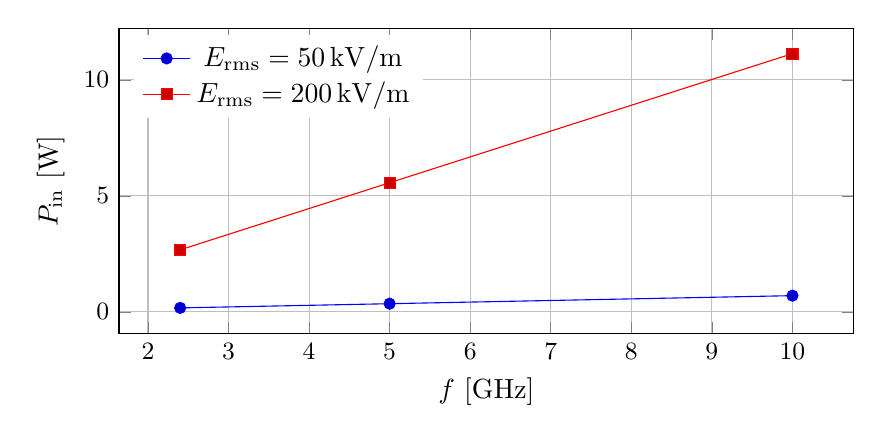
\begin{tikzpicture}
\begin{axis}[width=0.9\textwidth,height=0.45\textwidth, xlabel={$f$ [GHz]}, ylabel={$P_{\rm in}$ [W]},
    grid=both, legend style={at={(0.02,0.98)},anchor=north west,fill=white,draw=none}, ticklabel style={font=\small}]
\addplot+[mark=*] coordinates { (2.4, 0.167) (5.0, 0.348) (10.0, 0.695) };
\addlegendentry{$E_{\rm rms}=\SI{50}{kV/m}$}
\addplot+[mark=square*] coordinates { (2.4, 2.670) (5.0, 5.563) (10.0, 11.127) };
\addlegendentry{$E_{\rm rms}=\SI{200}{kV/m}$}
\end{axis}
\end{tikzpicture}
\caption{Drive power vs.\ frequency for two rms field levels in a $Q=10^6$ cavity of effective volume \SI{1e-3}{m^3}.}
\end{figure}

\section*{M.5 Safety and Operational Limits}
\textbf{Thermal and materials:} avoid excessive surface currents and ohmic heating; copper cavities at multi-GHz typically sustain tens of kV/m rms before significant heating; superconducting (SRF) cavities can exceed MV/m but demand cryogenics and strict cleanliness.
\medskip

\noindent\textbf{Breakdown:} vacuum breakdown fields are of order \SI{10^7}{V/m}--\SI{10^8}{V/m} at GHz under ideal surfaces; practical limits are lower due to asperities. Keep peak fields well below breakdown with safety factor $\ge 5$.
\medskip

\noindent\textbf{EMC and exposure:} operate in a shielded enclosure; ensure leakage below applicable RF exposure guidelines. Use interlocks and power ramp profiles. Keep biological SAR well within conservative limits (no human presence during high-power runs).

\section*{M.6 Detectability Window (Parametric)}
Let $\mathcal{K}_{\rm UBT}$ denote the net coupling from Appendix L so that $\Delta f/f \sim \mathcal{K}_{\rm UBT}\, U$ for a fixed mode (dimension absorbed in $\mathcal{K}_{\rm UBT}$).
Given metrological sensitivity $\sigma_{\Delta f/f}$ (e.g.\ $10^{-9}$--$10^{-7}$), the condition
\begin{equation}
U \gtrsim \frac{\sigma_{\Delta f/f}}{\mathcal{K}_{\rm UBT}}
\end{equation}
defines the minimal stored energy. With $Q$ fixed, $P_{\rm in}\propto f\,U$. Thus lower-$f$ modes minimize power for a given $U$, trading off cavity size.

\section*{M.7 Summary}
Under pure GR the metric response to laboratory EM energy is undetectably small. In UBT, a phase-sector weighting enables practical experiments within $\mathcal{O}(1)$--$10$~W drive for \SI{1e-3}{m^3} modes at $Q\!\sim\!10^6$, provided the $\psi$-sector is coherently engaged. Safety margins require shielding, interlocks, and conservative peak fields.
\end{document}
